\subsection{Loss Function}
\begin{frame}{}
	\LARGE VAE: \textbf{Loss Function}
\end{frame}

\begin{frame}[allowframebreaks]{Loss Function Breakdown}
\textbf{Total Loss:}
% This equation defines the loss function (L) for a Variational Autoencoder (VAE).
% The loss L is composed of two terms:
% 1. Reconstruction Loss: Measures how well the VAE reconstructs the input data.
% 2. KL Divergence: Regularizes the learned latent distribution to be close to a prior (usually a standard normal distribution).
% The symbol "L" here denotes the total VAE loss.
\[
L = \text{Reconstruction Loss} + \text{KL Divergence}
\]

\textbf{Reconstruction Loss:}
\begin{itemize}
    \item Measures how well $\hat{x}$ matches $x$.
    \item Common choices: Mean Squared Error (MSE) or Binary Cross-Entropy.
\end{itemize}

\textbf{KL Divergence:}
\begin{itemize}
    \item Measures how much $q(z \mid x)$ diverges from the prior $p(z)$.
    \item Encourages the latent space to follow a standard normal distribution.
\end{itemize}

\framebreak

\textbf{What if we trained with reconstruction only?}
\begin{itemize}
    \item The easiest way to reconstruct well is to be \textbf{deterministic}: the encoder shrinks $\sigma \to 0$ and the model degenerates into a plain autoencoder.
    \item Nothing constrains \textbf{where} the codes live: clusters drift far apart with empty space between them, and the decoder is undefined on the gaps.
    \item Sampling from $\mathcal{N}(0, I)$ then lands in regions the decoder has never seen; generation fails exactly as it did for the autoencoder.
    \item The KL term is what prevents both failures: it keeps $\sigma$ from collapsing and pulls all codes toward a shared, densely covered region around the origin.
\end{itemize}

\framebreak

\begin{figure}
    \centering
    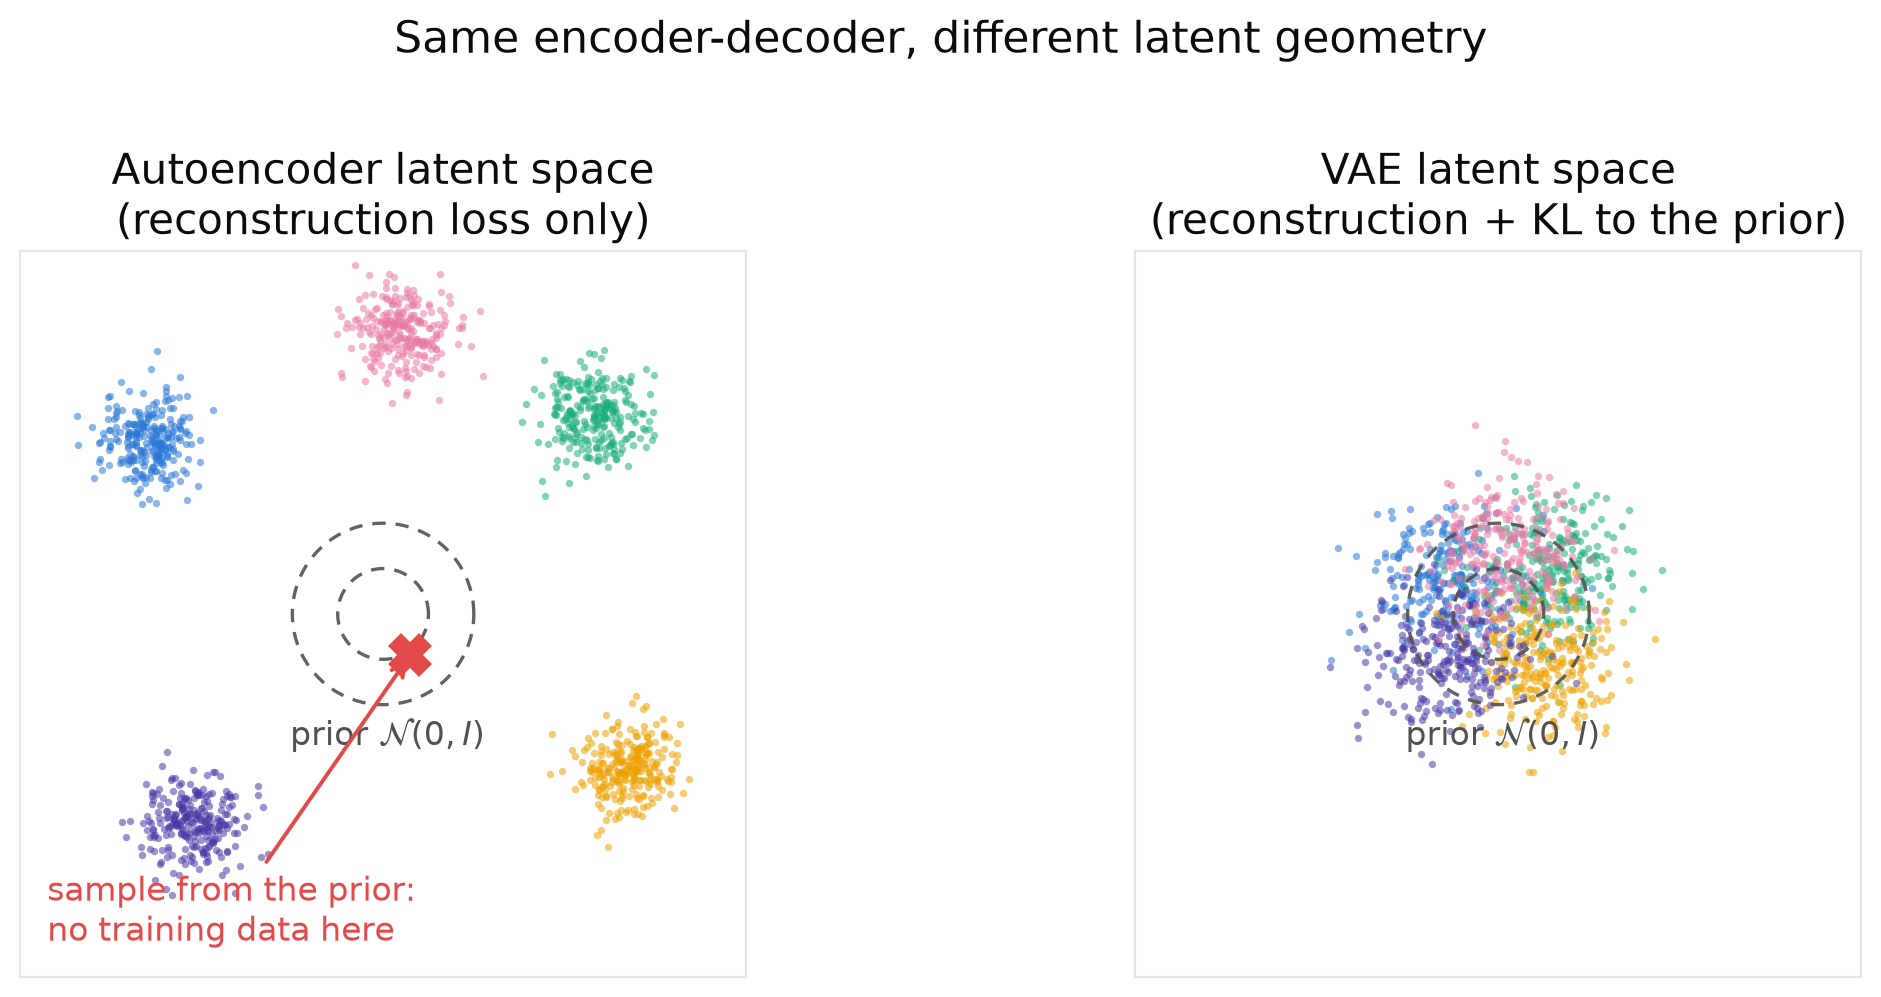
\includegraphics[height=0.72\textheight, width=\textwidth, keepaspectratio]{images/vae/latent_space_ae_vs_vae.png}
    \caption*{Reconstruction-only training scatters codes and leaves the prior in a hole (left); adding the KL term packs the posteriors around the prior so every sample decodes sensibly (right).}
\end{figure}
\end{frame}